\section{Eficiência Computacional e Trade-off Industrial}

No contexto da classificação industrial de algodão em tempo real, o desempenho preditivo deve ser equilibrado com o custo computacional e a latência de inferência. Um modelo com alta acurácia, mas latência proibitiva, inviabiliza sua implantação em esteiras automatizadas que processam múltiplas amostras por segundo.

A Figura \ref{fig:efficiency_tradeoff} ilustra o compromisso entre o \textit{Matthews Correlation Coefficient} (MCC), a latência média de inferência (em escala logarítmica) e a complexidade computacional em GFLOPs.

\begin{figure}[h!]
  \centering
  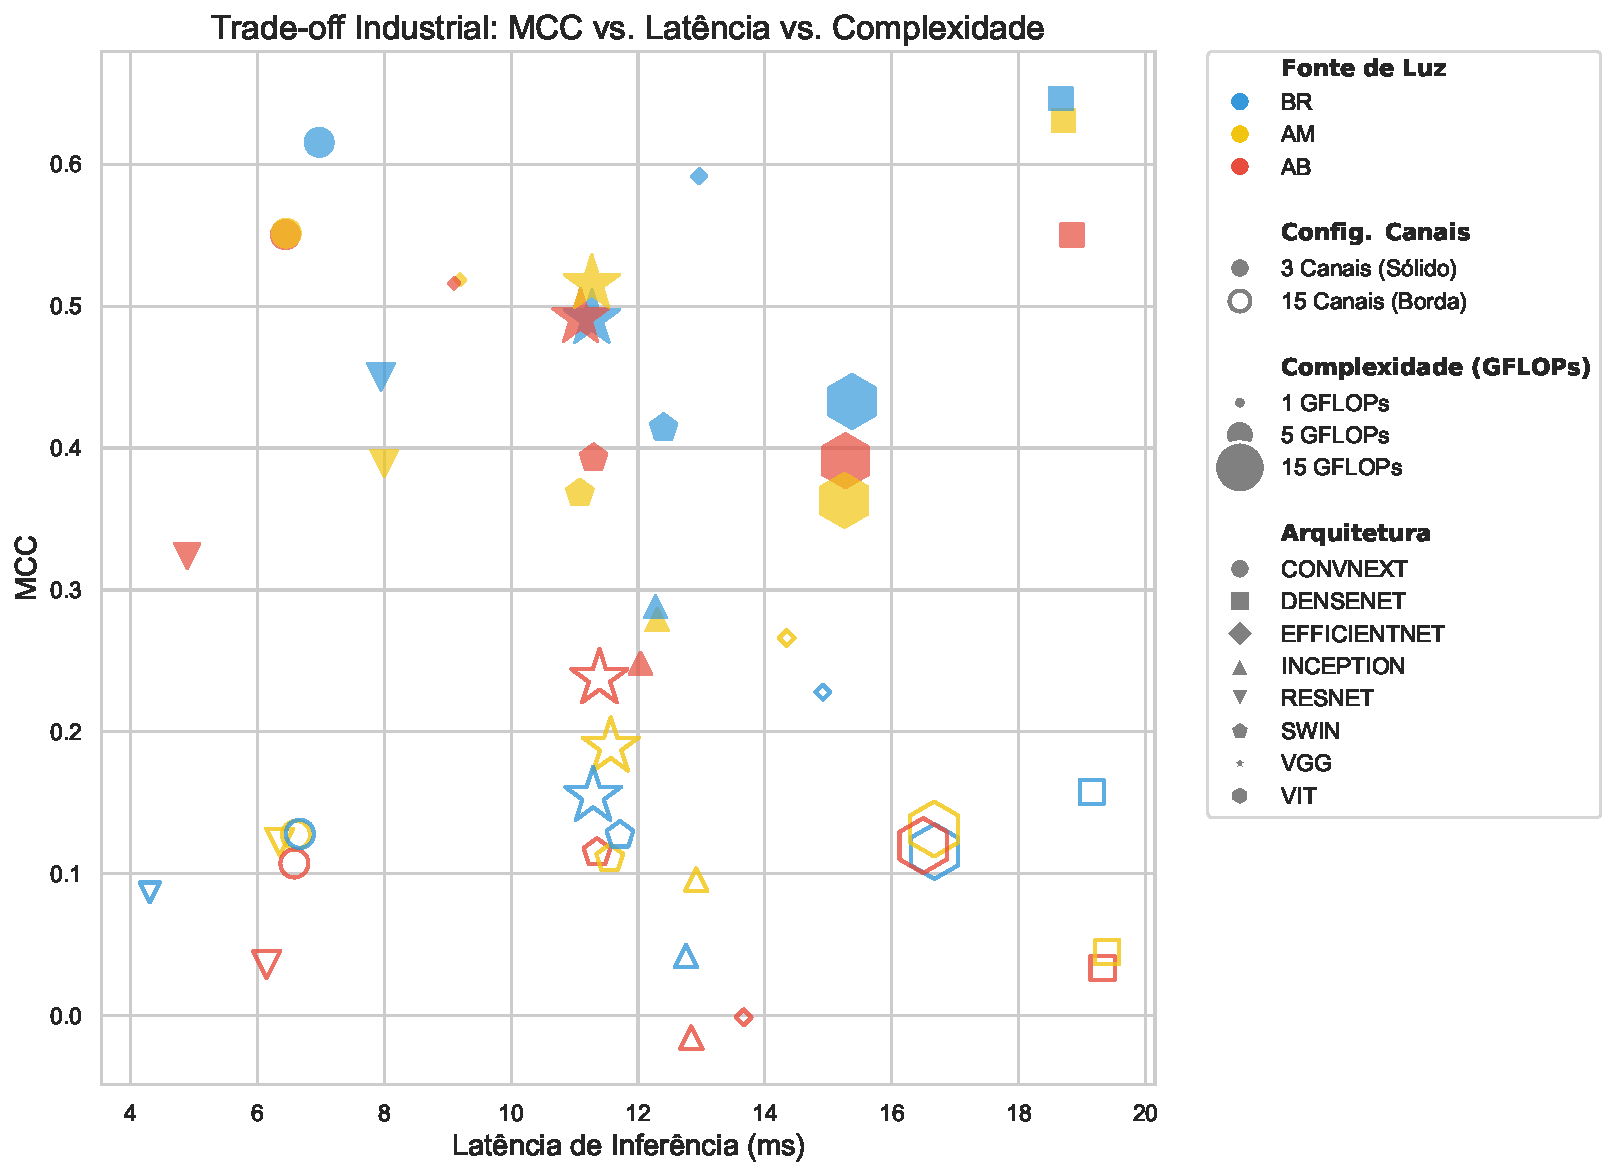
\includegraphics[width=1.0\textwidth]{images/efficiency_tradeoff_full.pdf}
  \caption{Trade-off Industrial: MCC vs. Latência (ms) vs. GFLOPs. O tamanho das bolhas representa a complexidade em GFLOPs.}
  \label{fig:efficiency_tradeoff}
\end{figure}

A análise revela que o modelo \textbf{ConvNext} oferece o melhor ponto de equilíbrio para aplicações de alta velocidade, apresentando uma latência de apenas \textbf{6,8 ms} com um MCC de 0,6153. Embora a \textbf{DenseNet} seja a mais precisa (MCC 0,6461), sua latência é quase três vezes superior (\textbf{19,4 ms}), o que pode limitar sua adoção em cenários de \textit{throughput} ultra-elevado.

Por outro lado, modelos como a \textbf{EfficientNet} (V10) mantêm-se competitivos com baixíssimo custo computacional (apenas 0,68 GFLOPs), sendo ideais para dispositivos de borda (\textit{edge computing}) ou sensores portáteis com recursos limitados. Em contrapartida, os modelos baseados em Vision Transformers (ViT) situam-se no quadrante menos eficiente do gráfico, com alta latência e alto consumo de memória paramétrica sem o retorno proporcional em performance preditiva para este dataset específico.
